%-------------------------------------------------------------------------------
% File:		    Presentation.tex
% Author:	    Igor Janjic, Danny Duangphachanh, Daniel Friedman
% Description:	[ECE 4564] Network Applications Design
%		        Project proposal presentation.
%%------------------------------------------------------------------------------ 

% Class options include: notes, notesonly, handout, trans, hidesubsections,
% shadesubsections, inrow, blue, red, grey, brown.
\documentclass[]{beamer}


% Theme for beamer presentation.
% Other themes include: beamerthemebars, beamerthemelined, beamerthemetree,
% beamerthemetreebars. 
\usepackage{beamerthemesplit}
\usepackage{caption}

\title{PiFeed - Feed Your Pets with a Raspberry Pi!}
\author{Daniel Friedman :: Igor Janjic :: Danny Duangphachanh}
\institute{Virginia Tech}
\date{\today}

\begin{document}

% Creates title page of slide show using above information.
\begin{frame}
  \titlepage
\end{frame}
\note{}

%\section[Outline]{}
%\begin{frame}
%	\frametitle{Outline}
%	\tableofcontents
%\end{frame}

\section{Objective}
\begin{frame}
	\frametitle{Objective}
    To create an automated cat and fish feeder with internet monitoring and control through the use of Raspberry Pi's
    \begin{itemize}
    	\item The ability to maintain a healthy eating schedule for pets is a concern for members of our group, as well as many others who travel or are away from home for an extended amount of time
        \item By successfully implementing a pet feeding and monitoring system using Raspberry Pi''s, the stresses of animal care while away will be a thing of the past!
    \end{itemize}
\end{frame}


% NEW SECTION
\section{Implementation}
\subsection{PiFeedControl}
\begin{frame}
	\frametitle{PiFeedControl}
    User will interface and be able to control the PiFeedFish/PiFeedCat remotely
    \begin{itemize}
    	\item Able to monitor both aquarium and cat feeder 
        \item Can customize feeders and control manually
    \end{itemize}
\end{frame}

\subsection{PiFeedFish/PiFeedCat}
\begin{frame}
	\frametitle{PiFeedFish}
    
    \begin{itemize}
    	\item Module to analyze sensor data
        \item Sends data when requested
        \item Controls feeder hardware
        \item Pi Camera to stream to a client
    \end{itemize}
\end{frame}

\subsection{Pictures}
\begin{frame}
	\begin{columns}[T]
    	\begin{column}{.5\textwidth}
        	\begin{block}{Cat Feeder}
				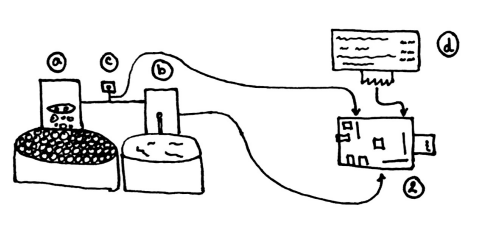
\includegraphics[width=\textwidth]{Cat}
            \end{block}
        \end{column}
        
    	\begin{column}{.5\textwidth}
        	\begin{block}{Fish Feeder}
            	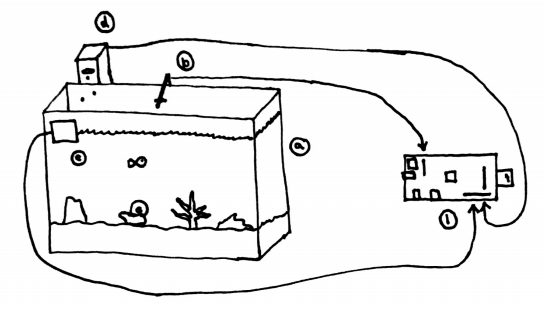
\includegraphics[width=\textwidth]{FishTank}
            \end{block}
        \end{column}
    \end{columns}
\end{frame}


% NEW SECTION
\section{IoT Patterns}
\begin{frame}
	\frametitle{IoT Net App Patterns}
	\begin{itemize}
    \item All sensor data will be published using RabbitMQ
    \item User control module will subscribe to the data
    \item User will access hardware/schedule events using sockets
    \end{itemize}
\end{frame}




% NEW SECTION
\section{Member Responsibilities}
\subsection{Everyone}
\begin{frame}
	\frametitle{Everyone}
	\begin{itemize}
    	\item Build automated fish tank feeder and automated cat feeder
        \item Test hardware component interfaces
        \item Test PiFeedControl, PiFeedFish, and PiFeedCat Python modules
        \item Test communication between all Raspberry Pi modules
        \item Demonstrate beta build and final build
    \end{itemize}
\end{frame}

\subsection{Danny}
\begin{frame}
	\frametitle{Danny}
	\begin{itemize}
    	\item Implement PiFeedCat and PiFeedFish Python modules
        \item Connect hardware components
    \end{itemize}
\end{frame}

\subsection{Daniel}
\begin{frame}
	\frametitle{Daniel}
	\begin{itemize}
    	\item Design automatedfish tank feeder and automated cat feeder
        \item Implement PiFeedControl python module
    \end{itemize}
\end{frame}

\subsection{Igor}
\begin{frame}
	\frametitle{Igor}
	\begin{itemize}
    	\item Design automated fish tank feeder and automated cat feeder
        \item Implement PiFeedControl, PiFeedCat, and PiFeedFish Python modules
    \end{itemize}
\end{frame}



% NEW SECTION
\section{Schedule}
\begin{frame}
	\frametitle{Gant Chart}
     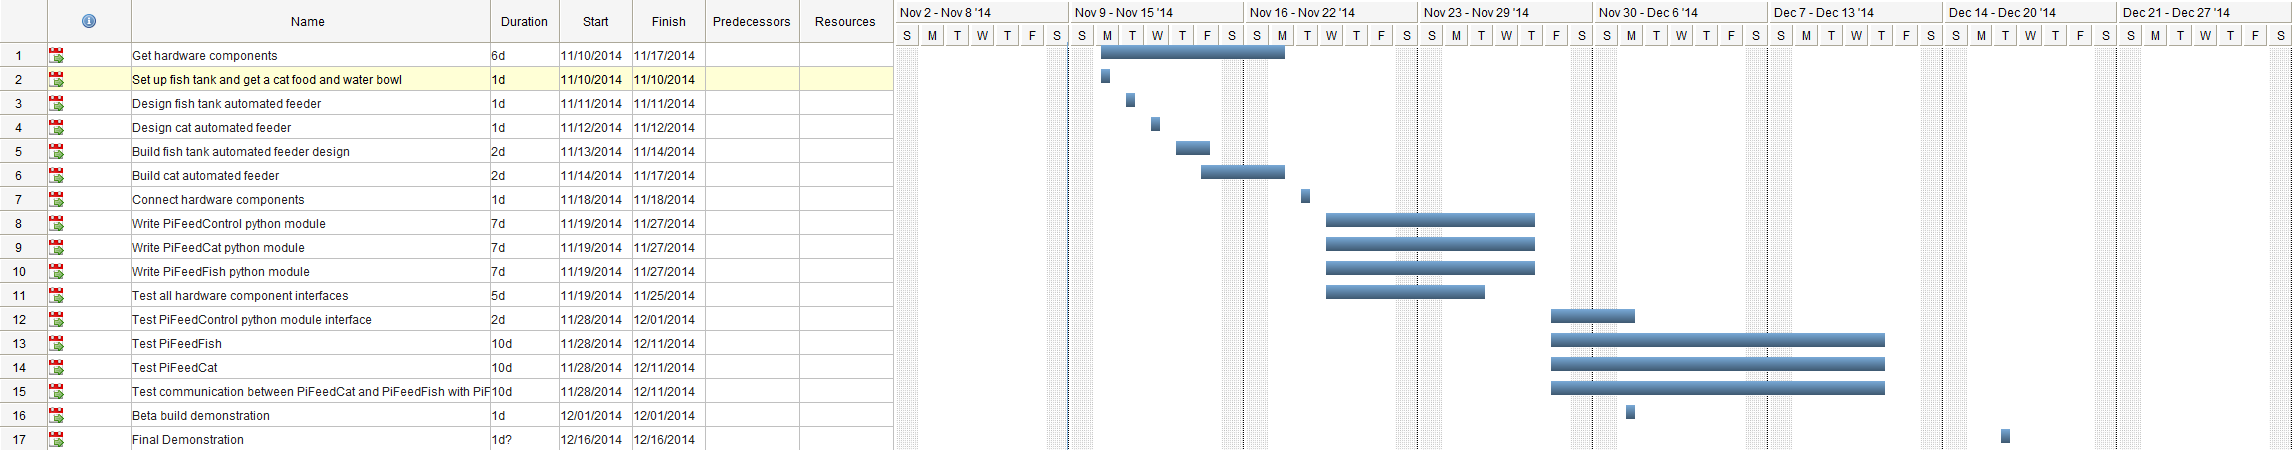
\includegraphics[width=\textwidth]{Gant}
\end{frame}



\end{document}
